% Options for packages loaded elsewhere
\PassOptionsToPackage{unicode}{hyperref}
\PassOptionsToPackage{hyphens}{url}
%
\documentclass[
]{article}
\usepackage{amsmath,amssymb}
\usepackage{lmodern}
\usepackage{iftex}
\ifPDFTeX
  \usepackage[T1]{fontenc}
  \usepackage[utf8]{inputenc}
  \usepackage{textcomp} % provide euro and other symbols
\else % if luatex or xetex
  \usepackage{unicode-math}
  \defaultfontfeatures{Scale=MatchLowercase}
  \defaultfontfeatures[\rmfamily]{Ligatures=TeX,Scale=1}
\fi
% Use upquote if available, for straight quotes in verbatim environments
\IfFileExists{upquote.sty}{\usepackage{upquote}}{}
\IfFileExists{microtype.sty}{% use microtype if available
  \usepackage[]{microtype}
  \UseMicrotypeSet[protrusion]{basicmath} % disable protrusion for tt fonts
}{}
\makeatletter
\@ifundefined{KOMAClassName}{% if non-KOMA class
  \IfFileExists{parskip.sty}{%
    \usepackage{parskip}
  }{% else
    \setlength{\parindent}{0pt}
    \setlength{\parskip}{6pt plus 2pt minus 1pt}}
}{% if KOMA class
  \KOMAoptions{parskip=half}}
\makeatother
\usepackage{xcolor}
\usepackage[margin=1in]{geometry}
\usepackage{color}
\usepackage{fancyvrb}
\newcommand{\VerbBar}{|}
\newcommand{\VERB}{\Verb[commandchars=\\\{\}]}
\DefineVerbatimEnvironment{Highlighting}{Verbatim}{commandchars=\\\{\}}
% Add ',fontsize=\small' for more characters per line
\usepackage{framed}
\definecolor{shadecolor}{RGB}{248,248,248}
\newenvironment{Shaded}{\begin{snugshade}}{\end{snugshade}}
\newcommand{\AlertTok}[1]{\textcolor[rgb]{0.94,0.16,0.16}{#1}}
\newcommand{\AnnotationTok}[1]{\textcolor[rgb]{0.56,0.35,0.01}{\textbf{\textit{#1}}}}
\newcommand{\AttributeTok}[1]{\textcolor[rgb]{0.77,0.63,0.00}{#1}}
\newcommand{\BaseNTok}[1]{\textcolor[rgb]{0.00,0.00,0.81}{#1}}
\newcommand{\BuiltInTok}[1]{#1}
\newcommand{\CharTok}[1]{\textcolor[rgb]{0.31,0.60,0.02}{#1}}
\newcommand{\CommentTok}[1]{\textcolor[rgb]{0.56,0.35,0.01}{\textit{#1}}}
\newcommand{\CommentVarTok}[1]{\textcolor[rgb]{0.56,0.35,0.01}{\textbf{\textit{#1}}}}
\newcommand{\ConstantTok}[1]{\textcolor[rgb]{0.00,0.00,0.00}{#1}}
\newcommand{\ControlFlowTok}[1]{\textcolor[rgb]{0.13,0.29,0.53}{\textbf{#1}}}
\newcommand{\DataTypeTok}[1]{\textcolor[rgb]{0.13,0.29,0.53}{#1}}
\newcommand{\DecValTok}[1]{\textcolor[rgb]{0.00,0.00,0.81}{#1}}
\newcommand{\DocumentationTok}[1]{\textcolor[rgb]{0.56,0.35,0.01}{\textbf{\textit{#1}}}}
\newcommand{\ErrorTok}[1]{\textcolor[rgb]{0.64,0.00,0.00}{\textbf{#1}}}
\newcommand{\ExtensionTok}[1]{#1}
\newcommand{\FloatTok}[1]{\textcolor[rgb]{0.00,0.00,0.81}{#1}}
\newcommand{\FunctionTok}[1]{\textcolor[rgb]{0.00,0.00,0.00}{#1}}
\newcommand{\ImportTok}[1]{#1}
\newcommand{\InformationTok}[1]{\textcolor[rgb]{0.56,0.35,0.01}{\textbf{\textit{#1}}}}
\newcommand{\KeywordTok}[1]{\textcolor[rgb]{0.13,0.29,0.53}{\textbf{#1}}}
\newcommand{\NormalTok}[1]{#1}
\newcommand{\OperatorTok}[1]{\textcolor[rgb]{0.81,0.36,0.00}{\textbf{#1}}}
\newcommand{\OtherTok}[1]{\textcolor[rgb]{0.56,0.35,0.01}{#1}}
\newcommand{\PreprocessorTok}[1]{\textcolor[rgb]{0.56,0.35,0.01}{\textit{#1}}}
\newcommand{\RegionMarkerTok}[1]{#1}
\newcommand{\SpecialCharTok}[1]{\textcolor[rgb]{0.00,0.00,0.00}{#1}}
\newcommand{\SpecialStringTok}[1]{\textcolor[rgb]{0.31,0.60,0.02}{#1}}
\newcommand{\StringTok}[1]{\textcolor[rgb]{0.31,0.60,0.02}{#1}}
\newcommand{\VariableTok}[1]{\textcolor[rgb]{0.00,0.00,0.00}{#1}}
\newcommand{\VerbatimStringTok}[1]{\textcolor[rgb]{0.31,0.60,0.02}{#1}}
\newcommand{\WarningTok}[1]{\textcolor[rgb]{0.56,0.35,0.01}{\textbf{\textit{#1}}}}
\usepackage{longtable,booktabs,array}
\usepackage{calc} % for calculating minipage widths
% Correct order of tables after \paragraph or \subparagraph
\usepackage{etoolbox}
\makeatletter
\patchcmd\longtable{\par}{\if@noskipsec\mbox{}\fi\par}{}{}
\makeatother
% Allow footnotes in longtable head/foot
\IfFileExists{footnotehyper.sty}{\usepackage{footnotehyper}}{\usepackage{footnote}}
\makesavenoteenv{longtable}
\usepackage{graphicx}
\makeatletter
\def\maxwidth{\ifdim\Gin@nat@width>\linewidth\linewidth\else\Gin@nat@width\fi}
\def\maxheight{\ifdim\Gin@nat@height>\textheight\textheight\else\Gin@nat@height\fi}
\makeatother
% Scale images if necessary, so that they will not overflow the page
% margins by default, and it is still possible to overwrite the defaults
% using explicit options in \includegraphics[width, height, ...]{}
\setkeys{Gin}{width=\maxwidth,height=\maxheight,keepaspectratio}
% Set default figure placement to htbp
\makeatletter
\def\fps@figure{htbp}
\makeatother
\setlength{\emergencystretch}{3em} % prevent overfull lines
\providecommand{\tightlist}{%
  \setlength{\itemsep}{0pt}\setlength{\parskip}{0pt}}
\setcounter{secnumdepth}{-\maxdimen} % remove section numbering
\ifLuaTeX
  \usepackage{selnolig}  % disable illegal ligatures
\fi
\IfFileExists{bookmark.sty}{\usepackage{bookmark}}{\usepackage{hyperref}}
\IfFileExists{xurl.sty}{\usepackage{xurl}}{} % add URL line breaks if available
\urlstyle{same} % disable monospaced font for URLs
\hypersetup{
  pdftitle={Assignment 1},
  pdfauthor={PD, JO, and MD, group 70},
  hidelinks,
  pdfcreator={LaTeX via pandoc}}

\title{Assignment 1}
\author{PD, JO, and MD, group 70}
\date{17 febuary 2023}

\begin{document}
\maketitle

\hypertarget{exercise-1}{%
\subsection{Exercise 1}\label{exercise-1}}

\begin{Shaded}
\begin{Highlighting}[]
\NormalTok{birthweight }\OtherTok{=} \FunctionTok{read.table}\NormalTok{(}\AttributeTok{file=}\StringTok{"../datasets/birthweight.txt"}\NormalTok{, }\AttributeTok{header=}\ConstantTok{FALSE}\NormalTok{)}
\NormalTok{birthweight }\OtherTok{\textless{}{-}}\NormalTok{ birthweight[}\DecValTok{2}\SpecialCharTok{:}\DecValTok{189}\NormalTok{,]}
\NormalTok{birthweight }\OtherTok{\textless{}{-}} \FunctionTok{as.numeric}\NormalTok{(}\FunctionTok{unlist}\NormalTok{(birthweight))}
\end{Highlighting}
\end{Shaded}

\textbf{a)} To check the data for normality we used a Shapiro-Wilk test.
This test tests the null hypothesis that a sample from an unknown
distribution is normal.

\begin{itemize}
\item
  Null hypothesis (H0): The mean weight is the same for male and female
  babies.
\item
  Alternative hypothesis (Ha): The mean weight is different for male and
  female babies.
\end{itemize}

Our p-value of 0.90 is higher then the confidence level of 0.05 this
means we cannot reject our null hypothesis. This hypothesis is
complemented by the QQ-plot and histogram of the data that both
approximate a normal distribution.

\begin{Shaded}
\begin{Highlighting}[]
\CommentTok{\# check normality}
\FunctionTok{shapiro.test}\NormalTok{(birthweight)}
\end{Highlighting}
\end{Shaded}

\begin{verbatim}
## 
##  Shapiro-Wilk normality test
## 
## data:  birthweight
## W = 0.99595, p-value = 0.8995
\end{verbatim}

\begin{Shaded}
\begin{Highlighting}[]
\FunctionTok{par}\NormalTok{(}\AttributeTok{mfrow=}\FunctionTok{c}\NormalTok{(}\DecValTok{1}\NormalTok{,}\DecValTok{2}\NormalTok{))}
\FunctionTok{qqnorm}\NormalTok{(birthweight)}
\FunctionTok{hist}\NormalTok{(birthweight)}
\end{Highlighting}
\end{Shaded}

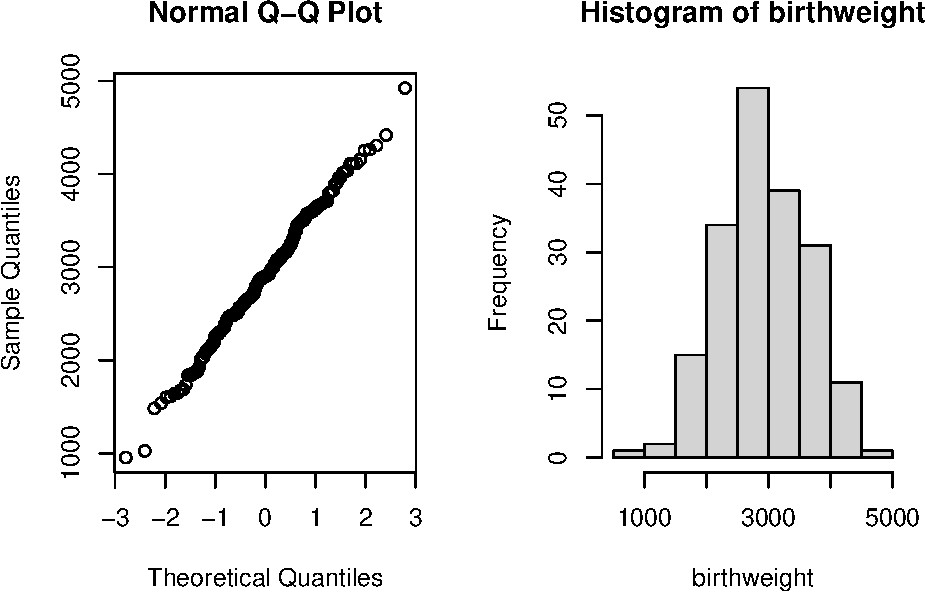
\includegraphics{assignment_1_files/figure-latex/unnamed-chunk-2-1.pdf}

Assuming normality we can construct a 96\%-CI for the mean. We
constructed the CI using a t-test with a confidence level of 0.96. The
resulting confidence interval is {[}2808.08, 3018,50{]}.

\begin{Shaded}
\begin{Highlighting}[]
\CommentTok{\# 96\%{-}CI}
\NormalTok{m }\OtherTok{=} \FunctionTok{mean}\NormalTok{(birthweight)}
\FunctionTok{t.test}\NormalTok{(birthweight, }\AttributeTok{mu=}\NormalTok{m, }\AttributeTok{conf.level =} \FloatTok{0.96}\NormalTok{)}
\end{Highlighting}
\end{Shaded}

\begin{verbatim}
## 
##  One Sample t-test
## 
## data:  birthweight
## t = 0, df = 187, p-value = 1
## alternative hypothesis: true mean is not equal to 2913.293
## 96 percent confidence interval:
##  2808.084 3018.501
## sample estimates:
## mean of x 
##  2913.293
\end{verbatim}

The sample size needed to provide that the length of the CI is at most
100, is the sample size needed to get a CI of μ +/- 100/2. The sample
size necessary is 550.

\begin{Shaded}
\begin{Highlighting}[]
\CommentTok{\#sample size needed for CI length of 100}
\NormalTok{e }\OtherTok{=} \DecValTok{100}\SpecialCharTok{/}\FunctionTok{mean}\NormalTok{(birthweight)}
\FunctionTok{qnorm}\NormalTok{(}\FloatTok{0.98}\NormalTok{)}\SpecialCharTok{\^{}}\DecValTok{2}\SpecialCharTok{*}\FloatTok{0.96}\SpecialCharTok{*}\FloatTok{0.04}\SpecialCharTok{/}\NormalTok{(e}\SpecialCharTok{/}\DecValTok{2}\NormalTok{)}\SpecialCharTok{\^{}}\DecValTok{2}
\end{Highlighting}
\end{Shaded}

\begin{verbatim}
## [1] 549.8625
\end{verbatim}

The bootstrap CI is very similar to the CI that we got with the t-test
it is just a fraction smaller. Which could mean that the bootstrap
interval is more robust than the t-test interval.

\begin{Shaded}
\begin{Highlighting}[]
\CommentTok{\#bootstrap}
\NormalTok{B}\OtherTok{=}\DecValTok{1000}
\NormalTok{Tstar }\OtherTok{=} \FunctionTok{numeric}\NormalTok{(B)}
\ControlFlowTok{for}\NormalTok{(i }\ControlFlowTok{in} \DecValTok{1}\SpecialCharTok{:}\NormalTok{B)\{}
\NormalTok{  Xstar }\OtherTok{=} \FunctionTok{sample}\NormalTok{(birthweight, }\AttributeTok{replace=}\ConstantTok{TRUE}\NormalTok{)}
\NormalTok{  Tstar[i] }\OtherTok{=} \FunctionTok{mean}\NormalTok{(Xstar)}
\NormalTok{\}}
\NormalTok{Tstar2 }\OtherTok{=} \FunctionTok{quantile}\NormalTok{(Tstar, }\FloatTok{0.02}\NormalTok{)}
\NormalTok{Tstar98 }\OtherTok{=} \FunctionTok{quantile}\NormalTok{(Tstar, }\FloatTok{0.98}\NormalTok{)}
\FunctionTok{sum}\NormalTok{(Tstar}\SpecialCharTok{\textless{}}\NormalTok{Tstar2)}
\end{Highlighting}
\end{Shaded}

\begin{verbatim}
## [1] 20
\end{verbatim}

\begin{Shaded}
\begin{Highlighting}[]
\FunctionTok{c}\NormalTok{(}\DecValTok{2}\SpecialCharTok{*}\NormalTok{m }\SpecialCharTok{{-}}\NormalTok{ Tstar98, }\DecValTok{2}\SpecialCharTok{*}\NormalTok{m }\SpecialCharTok{{-}}\NormalTok{ Tstar2)}
\end{Highlighting}
\end{Shaded}

\begin{verbatim}
##      98%       2% 
## 2807.423 3028.833
\end{verbatim}

\textbf{b)}

To verify the claim we do a t-test with H0: μ = 2800 and Ha: μ
\textgreater{} 2800. The result of the t-test has a p-value of 0.014,
which is smaller than alpha. This means we can reject H0, and Ha is
accepted. The test also tells us that there is a probability of 95\%
that the mean is greater than 2819.20. For an appropriate sign-test we
check the number of observations that are greater than 2800 and the
total number of observations in the data set. With H0: μ = 2800 and Ha:
μ \textgreater{} 2800. The result of the sign-test has a p-value of
0.033, so H0 is rejected. The results tell us that the number of
observations that are greater than 2800 is greater than the number of
total observations divided by two.

\begin{Shaded}
\begin{Highlighting}[]
\CommentTok{\#t{-}test to verify mean weight is bigger than 2800}
\FunctionTok{t.test}\NormalTok{(birthweight, }\AttributeTok{mu=}\DecValTok{2800}\NormalTok{, }\AttributeTok{alternative =} \StringTok{"g"}\NormalTok{)}
\end{Highlighting}
\end{Shaded}

\begin{verbatim}
## 
##  One Sample t-test
## 
## data:  birthweight
## t = 2.2271, df = 187, p-value = 0.01357
## alternative hypothesis: true mean is greater than 2800
## 95 percent confidence interval:
##  2829.202      Inf
## sample estimates:
## mean of x 
##  2913.293
\end{verbatim}

\begin{Shaded}
\begin{Highlighting}[]
\CommentTok{\#sign test}
\FunctionTok{binom.test}\NormalTok{(}\FunctionTok{sum}\NormalTok{(birthweight}\SpecialCharTok{\textgreater{}}\DecValTok{2800}\NormalTok{), }\FunctionTok{length}\NormalTok{(birthweight), }\AttributeTok{alternative =} \StringTok{"g"}\NormalTok{)}
\end{Highlighting}
\end{Shaded}

\begin{verbatim}
## 
##  Exact binomial test
## 
## data:  sum(birthweight > 2800) and length(birthweight)
## number of successes = 107, number of trials = 188, p-value = 0.03399
## alternative hypothesis: true probability of success is greater than 0.5
## 95 percent confidence interval:
##  0.5065781 1.0000000
## sample estimates:
## probability of success 
##              0.5691489
\end{verbatim}

\textbf{c)}

We can test the power of the test by simulation. By generating data and
checking the fraction of the sample where H0 is rejected. The powers of
the test tell us that the t-test performs better than the sign-test.
This is because the sign-test is a non-parametric test, which means it
makes very few assumption about the data but this can also lead to a
lack of statistical power.

\begin{Shaded}
\begin{Highlighting}[]
\CommentTok{\#geen idee of dit goed is}
\CommentTok{\#power of t{-}test and sign test}
\NormalTok{B}\OtherTok{=}\DecValTok{10000}\NormalTok{; n}\OtherTok{=}\DecValTok{188}\NormalTok{; s }\OtherTok{=} \FunctionTok{sd}\NormalTok{(birthweight); m }\OtherTok{=} \FunctionTok{mean}\NormalTok{(birthweight)}
\NormalTok{psign }\OtherTok{=} \FunctionTok{numeric}\NormalTok{(B)}
\NormalTok{pttest }\OtherTok{=} \FunctionTok{numeric}\NormalTok{(B)}

\ControlFlowTok{for}\NormalTok{(i }\ControlFlowTok{in} \DecValTok{1}\SpecialCharTok{:}\NormalTok{B)\{}
\NormalTok{  x }\OtherTok{=} \FunctionTok{rnorm}\NormalTok{(n, }\AttributeTok{mean=}\NormalTok{m, }\AttributeTok{sd=}\NormalTok{s)}
\NormalTok{  pttest[i] }\OtherTok{=} \FunctionTok{t.test}\NormalTok{(x, }\AttributeTok{mu=}\DecValTok{2800}\NormalTok{, }\AttributeTok{alternative =} \StringTok{"g"}\NormalTok{)[[}\DecValTok{3}\NormalTok{]]}
\NormalTok{  psign[i] }\OtherTok{=} \FunctionTok{binom.test}\NormalTok{(}\FunctionTok{sum}\NormalTok{(x}\SpecialCharTok{\textgreater{}}\DecValTok{2800}\NormalTok{), n, }\AttributeTok{alternative =}\StringTok{"g"}\NormalTok{)[[}\DecValTok{3}\NormalTok{]]}
\NormalTok{\}}

\FunctionTok{sum}\NormalTok{(pttest}\SpecialCharTok{\textless{}}\FloatTok{0.05}\NormalTok{)}\SpecialCharTok{/}\NormalTok{B}
\end{Highlighting}
\end{Shaded}

\begin{verbatim}
## [1] 0.7143
\end{verbatim}

\begin{Shaded}
\begin{Highlighting}[]
\FunctionTok{sum}\NormalTok{(psign}\SpecialCharTok{\textless{}}\FloatTok{0.05}\NormalTok{)}\SpecialCharTok{/}\NormalTok{B}
\end{Highlighting}
\end{Shaded}

\begin{verbatim}
## [1] 0.5422
\end{verbatim}

\textbf{d)}

The confidence interval for P(X\textless2600) is {[}0.25, 0.41{]}, with
a confidence level of 0.98.

\begin{Shaded}
\begin{Highlighting}[]
\NormalTok{n }\OtherTok{=} \FunctionTok{length}\NormalTok{(birthweight)}
\NormalTok{lower\_bound }\OtherTok{=} \FloatTok{0.25}
\NormalTok{p\_hat }\OtherTok{=} \FunctionTok{sum}\NormalTok{(birthweight}\SpecialCharTok{\textless{}}\DecValTok{2600}\NormalTok{)}\SpecialCharTok{/}\NormalTok{n}
\NormalTok{margin }\OtherTok{=}\NormalTok{ p\_hat }\SpecialCharTok{{-}}\NormalTok{ lower\_bound}
\NormalTok{upper\_bound }\OtherTok{=}\NormalTok{ lower\_bound }\SpecialCharTok{+} \DecValTok{2}\SpecialCharTok{*}\NormalTok{margin}
\NormalTok{z }\OtherTok{=}\NormalTok{ margin }\SpecialCharTok{/} \FunctionTok{sqrt}\NormalTok{((p\_hat}\SpecialCharTok{*}\NormalTok{(}\DecValTok{1}\SpecialCharTok{{-}}\NormalTok{p\_hat))}\SpecialCharTok{/}\NormalTok{n)}
\NormalTok{alpha }\OtherTok{=}\NormalTok{ (}\DecValTok{1} \SpecialCharTok{{-}} \FunctionTok{pnorm}\NormalTok{(z))}\SpecialCharTok{*}\DecValTok{2}
\NormalTok{confidence\_level }\OtherTok{=} \DecValTok{1} \SpecialCharTok{{-}}\NormalTok{ alpha}
\end{Highlighting}
\end{Shaded}

\textbf{e)}

To test the claim that there is a difference in the mean birth weight of
male and female babies are different we can perform a prop test on the
proportions of males and females that are born with a weight below 2600
gram.

\begin{itemize}
\item
  Null hypothesis (H0) : There is no difference in proportion between
  male and female babies born with a weight less than 2600.
\item
  Alternative hypothesis (Ha) : There is a difference in proportion
  between male and female babies born with a weight less than 2600.
\end{itemize}

This test concludes with a p-value of \textasciitilde0.5 and therefore
we cannot reject the null hypothesis.

We can not directly reject the claim that there is a difference in the
mean birth weight between male and female babies because we cannot
directly measure this. However, we also have not found evidence for it
in the given proportions.

\begin{Shaded}
\begin{Highlighting}[]
\NormalTok{male\_weights }\OtherTok{\textless{}{-}} \FunctionTok{c}\NormalTok{(}\DecValTok{34}\NormalTok{, }\DecValTok{61}\NormalTok{)}
\NormalTok{female\_weights }\OtherTok{\textless{}{-}} \FunctionTok{c}\NormalTok{(}\DecValTok{28}\NormalTok{, }\DecValTok{65}\NormalTok{)}

\NormalTok{x}\OtherTok{\textless{}{-}}\FunctionTok{c}\NormalTok{(male\_weights[}\DecValTok{1}\NormalTok{],female\_weights[}\DecValTok{1}\NormalTok{])}
\NormalTok{y}\OtherTok{\textless{}{-}}\FunctionTok{c}\NormalTok{(}\FunctionTok{sum}\NormalTok{(male\_weights),}\FunctionTok{sum}\NormalTok{(female\_weights))}

\FunctionTok{prop.test}\NormalTok{(x, y)}
\end{Highlighting}
\end{Shaded}

\begin{verbatim}
## 
##  2-sample test for equality of proportions with continuity correction
## 
## data:  x out of y
## X-squared = 0.45343, df = 1, p-value = 0.5007
## alternative hypothesis: two.sided
## 95 percent confidence interval:
##  -0.08792638  0.20156532
## sample estimates:
##    prop 1    prop 2 
## 0.3578947 0.3010753
\end{verbatim}

\hypertarget{exercise-2}{%
\subsection{Exercise 2}\label{exercise-2}}

\begin{Shaded}
\begin{Highlighting}[]
\NormalTok{fat }\OtherTok{=} \FunctionTok{scan}\NormalTok{(}\StringTok{"../datasets/cholesterol.txt"}\NormalTok{, }\AttributeTok{what =} \FunctionTok{list}\NormalTok{(}\AttributeTok{before =} \DecValTok{0}\NormalTok{, }\AttributeTok{after =} \DecValTok{0}\NormalTok{));}
\FunctionTok{attach}\NormalTok{(fat);}
\end{Highlighting}
\end{Shaded}

\textbf{a)}

To investigate the data set we create a box plot of both columns.
Judging from this we can observe a possible difference. The mean of the
data from after 8 weeks appears to be lower.

\begin{Shaded}
\begin{Highlighting}[]
\FunctionTok{boxplot}\NormalTok{(fat)}
\end{Highlighting}
\end{Shaded}

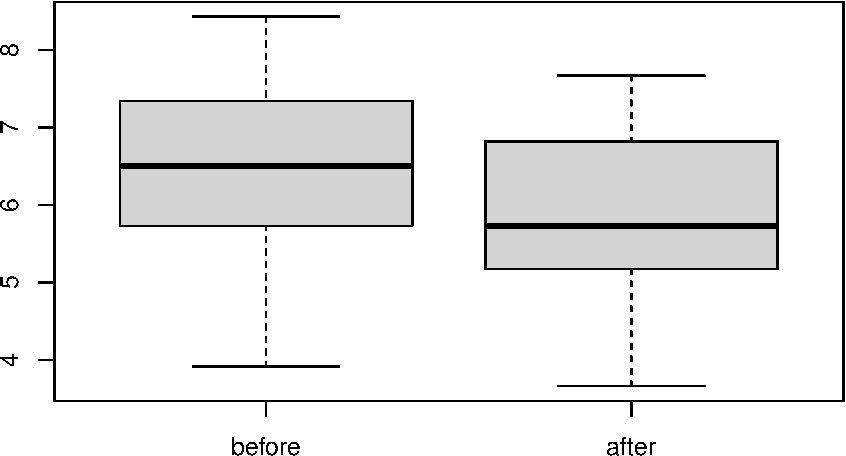
\includegraphics{assignment_1_files/figure-latex/unnamed-chunk-11-1.pdf}

Next we plot a normal Q-Q plot to check if the data is normally
distributed. this appears to be the case.

\begin{Shaded}
\begin{Highlighting}[]
\FunctionTok{par}\NormalTok{(}\AttributeTok{mfrow =} \FunctionTok{c}\NormalTok{(}\DecValTok{1}\NormalTok{,}\DecValTok{2}\NormalTok{)); }\FunctionTok{qqnorm}\NormalTok{(before); }\FunctionTok{qqnorm}\NormalTok{(after)}
\end{Highlighting}
\end{Shaded}

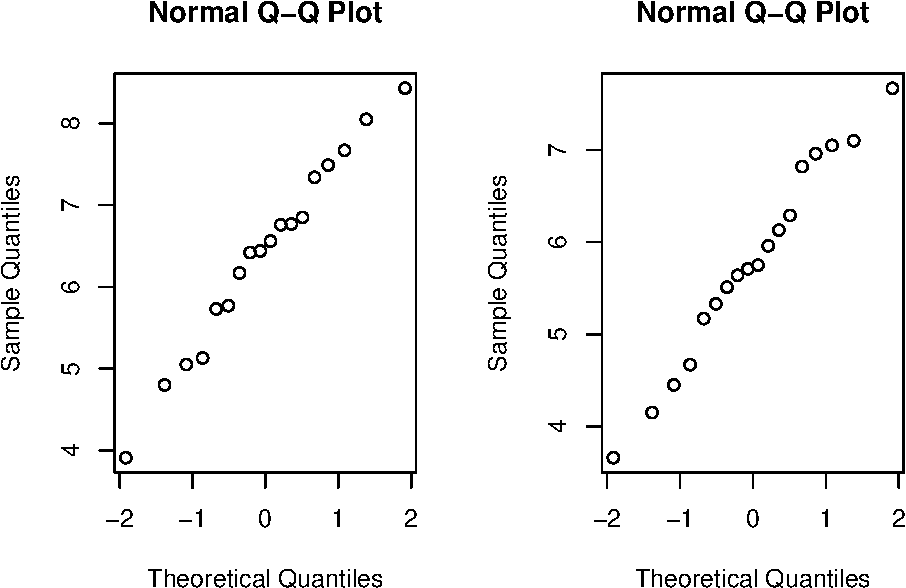
\includegraphics{assignment_1_files/figure-latex/unnamed-chunk-12-1.pdf}

To check if the before and after 8 weeks data is correlated we can plot
the two data sets against each other. The plot shows a clear linear
correlation between before and after. Then we can confirm this with both
the Pearson's and Spearman's correlation test. Both of these give the
conclusion that there indeed is a correlation and it is a strong
correlation with \textbf{an r value of 0.99.}

\begin{Shaded}
\begin{Highlighting}[]
\FunctionTok{plot}\NormalTok{(before}\SpecialCharTok{\textasciitilde{}}\NormalTok{after)}
\end{Highlighting}
\end{Shaded}

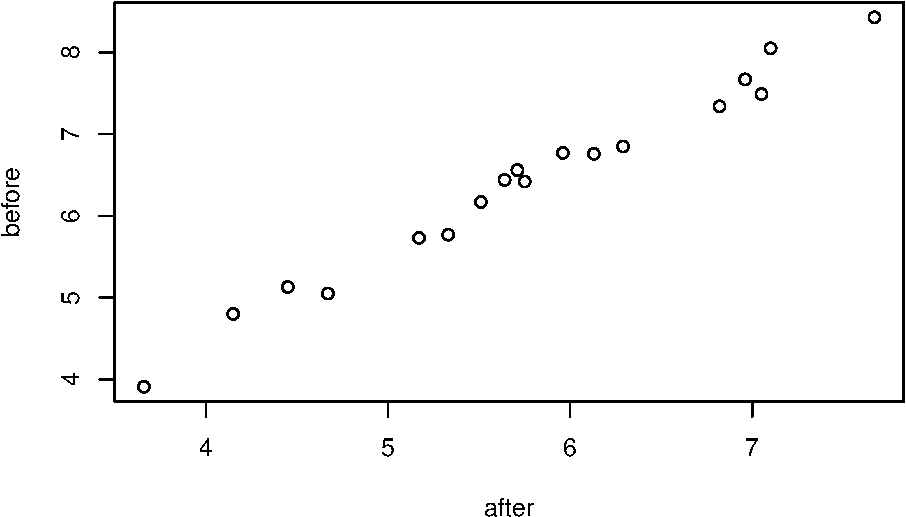
\includegraphics{assignment_1_files/figure-latex/unnamed-chunk-13-1.pdf}

\begin{Shaded}
\begin{Highlighting}[]
\FunctionTok{cor.test}\NormalTok{(before, after)}
\end{Highlighting}
\end{Shaded}

\begin{verbatim}
## 
##  Pearson's product-moment correlation
## 
## data:  before and after
## t = 29.428, df = 16, p-value = 2.321e-15
## alternative hypothesis: true correlation is not equal to 0
## 95 percent confidence interval:
##  0.9751289 0.9966788
## sample estimates:
##       cor 
## 0.9908885
\end{verbatim}

\begin{Shaded}
\begin{Highlighting}[]
\FunctionTok{cor.test}\NormalTok{(before, after, }\AttributeTok{method=}\StringTok{"spearman"}\NormalTok{)}
\end{Highlighting}
\end{Shaded}

\begin{verbatim}
## 
##  Spearman's rank correlation rho
## 
## data:  before and after
## S = 12, p-value = 9.753e-06
## alternative hypothesis: true rho is not equal to 0
## sample estimates:
##       rho 
## 0.9876161
\end{verbatim}

\textbf{b)}

Since the data is collected from the same patient before and after 8
weeks it is clear the data is paired. We can therefore perform a t-test
to investigate whether there is a difference in the mean of the before
and after data.

\begin{itemize}
\tightlist
\item
  Null hypothesis (H0) : mean(before) = mean(after)
\item
  Alternative hypothesis (Ha) : mean(before) \textgreater{} mean(after)
\end{itemize}

Performing a t.test gives us a p-value of 1.639e-11 this is smaller than
our significance level of 0.05 and we can therefore reject the null
hypothesis. The before data has a mean that is greater than the mean of
the after data.

\begin{Shaded}
\begin{Highlighting}[]
\FunctionTok{t.test}\NormalTok{(before, after, }\AttributeTok{alternative=}\StringTok{"greater"}\NormalTok{, }\AttributeTok{paired =} \ConstantTok{TRUE}\NormalTok{)}
\end{Highlighting}
\end{Shaded}

\begin{verbatim}
## 
##  Paired t-test
## 
## data:  before and after
## t = 14.946, df = 17, p-value = 1.639e-11
## alternative hypothesis: true mean difference is greater than 0
## 95 percent confidence interval:
##  0.5556906       Inf
## sample estimates:
## mean difference 
##       0.6288889
\end{verbatim}

We also perform a Wilcoxon signed rank test to check if the same
conclusion can be drawn. The test gives us a p-value of 3.815e-06. with
significance level of 0.05 we can reject the null hypothesis again.

\begin{Shaded}
\begin{Highlighting}[]
\FunctionTok{wilcox.test}\NormalTok{(before, after, }\AttributeTok{alternative =} \StringTok{"greater"}\NormalTok{, }\AttributeTok{paired =} \ConstantTok{TRUE}\NormalTok{)}
\end{Highlighting}
\end{Shaded}

\begin{verbatim}
## 
##  Wilcoxon signed rank exact test
## 
## data:  before and after
## V = 171, p-value = 3.815e-06
## alternative hypothesis: true location shift is greater than 0
\end{verbatim}

A permutation test is applicable for independent samples with any test
statistic that expresses difference between the samples. This means that
for the before and after data we can perform this test is the data is
independent. The before and after data are independent therefore we
might perform a permutation test.

\textbf{c)}

The estimator of θ we find by computing max(after). Now we can find the
confidence interval for this estimator by the bootstrapped confidence
interval method. This gives us a confidence interval of {[}7.67, 8.38{]}

\begin{Shaded}
\begin{Highlighting}[]
\NormalTok{B}\OtherTok{=}\DecValTok{1000}
\NormalTok{T1 }\OtherTok{=} \FunctionTok{max}\NormalTok{(after)}
\NormalTok{Tstar}\OtherTok{=}\FunctionTok{numeric}\NormalTok{(B)}
\NormalTok{c1 }\OtherTok{=}\NormalTok{ after}

\ControlFlowTok{for}\NormalTok{(i }\ControlFlowTok{in} \DecValTok{1}\SpecialCharTok{:}\NormalTok{B) \{}
\NormalTok{  Xstar}\OtherTok{=}\FunctionTok{sample}\NormalTok{(c1,}\AttributeTok{replace=}\ConstantTok{TRUE}\NormalTok{)}
\NormalTok{  Tstar[i]}\OtherTok{=}\FunctionTok{max}\NormalTok{(Xstar)}
\NormalTok{\}}
\NormalTok{Tstar25}\OtherTok{=}\FunctionTok{quantile}\NormalTok{(Tstar,}\FloatTok{0.025}\NormalTok{)}
\NormalTok{Tstar975}\OtherTok{=}\FunctionTok{quantile}\NormalTok{(Tstar,}\FloatTok{0.975}\NormalTok{)}

\FunctionTok{c}\NormalTok{(}\DecValTok{2}\SpecialCharTok{*}\NormalTok{T1}\SpecialCharTok{{-}}\NormalTok{Tstar975,}\DecValTok{2}\SpecialCharTok{*}\NormalTok{T1}\SpecialCharTok{{-}}\NormalTok{Tstar25)}
\end{Highlighting}
\end{Shaded}

\begin{verbatim}
## 97.5%  2.5% 
##  7.67  8.38
\end{verbatim}

\textbf{d)}

To determine for which θs we cannot reject that our estimate

\begin{itemize}
\item
  Null hypothesis (H0): p(after) = unif(3,θ) where θ in {[}3, 12{]}
\item
  Alternative hypothesis (Ha): p(after) ≠ unif(3,θ) where θ in {[}3,
  12{]}
\end{itemize}

We performed the bootstrap test for the values for θ in 3 \ldots{} 12.
For the values inside the bootstrapped confidence interval we cannot
reject the null hypothesis.

the Kolmogorov-Smirnoff (KS) test can be used to perform this analysis.
This can be done by generating data from the uniform distribution and
performing the KS test on the generated data and the after data.

\begin{Shaded}
\begin{Highlighting}[]
\NormalTok{data }\OtherTok{=}\NormalTok{ after}
\NormalTok{n}\OtherTok{=}\FunctionTok{length}\NormalTok{(data); t}\OtherTok{=}\FunctionTok{max}\NormalTok{(data); t}
\end{Highlighting}
\end{Shaded}

\begin{verbatim}
## [1] 7.67
\end{verbatim}

\begin{Shaded}
\begin{Highlighting}[]
\NormalTok{B}\OtherTok{=}\DecValTok{1000}\NormalTok{; tstar}\OtherTok{=}\FunctionTok{numeric}\NormalTok{(B)}
\ControlFlowTok{for}\NormalTok{ (i }\ControlFlowTok{in} \DecValTok{1}\SpecialCharTok{:}\NormalTok{B) \{}
\NormalTok{  xstar}\OtherTok{=}\FunctionTok{runif}\NormalTok{(n, }\DecValTok{3}\NormalTok{, }\DecValTok{9}\NormalTok{)}
\NormalTok{  tstar[i]}\OtherTok{=}\FunctionTok{max}\NormalTok{(xstar)}
\NormalTok{\}}

\NormalTok{pl}\OtherTok{=}\FunctionTok{sum}\NormalTok{(tstar}\SpecialCharTok{\textless{}}\NormalTok{t)}\SpecialCharTok{/}\NormalTok{B;}
\NormalTok{pr}\OtherTok{=}\FunctionTok{sum}\NormalTok{(tstar}\SpecialCharTok{\textgreater{}}\NormalTok{t)}\SpecialCharTok{/}\NormalTok{B}
\NormalTok{p}\OtherTok{=}\DecValTok{2}\SpecialCharTok{*}\FunctionTok{min}\NormalTok{(pl,pr); p}
\end{Highlighting}
\end{Shaded}

\begin{verbatim}
## [1] 0.018
\end{verbatim}

\textbf{e)}

Using the sign test we are test if H0: median(after) = 6. with Ha:
median(after ) \textless{} 6. Performing the test gives us a p-value of
0.61111 this is not lower than our significance level of 0.05 and
therefore we cannot reject the null hypothesis.

\begin{Shaded}
\begin{Highlighting}[]
\NormalTok{x }\OtherTok{=} \FunctionTok{sum}\NormalTok{(after}\SpecialCharTok{\textless{}}\DecValTok{6}\NormalTok{)}
\NormalTok{n }\OtherTok{=} \FunctionTok{length}\NormalTok{(after}\SpecialCharTok{\textless{}}\DecValTok{6}\NormalTok{)}
\FunctionTok{binom.test}\NormalTok{(x, n, x}\SpecialCharTok{/}\NormalTok{n, }\StringTok{"l"}\NormalTok{)}
\end{Highlighting}
\end{Shaded}

\begin{verbatim}
## 
##  Exact binomial test
## 
## data:  x and n
## number of successes = 11, number of trials = 18, p-value = 0.5883
## alternative hypothesis: true probability of success is less than 0.6111111
## 95 percent confidence interval:
##  0.0000000 0.8010467
## sample estimates:
## probability of success 
##              0.6111111
\end{verbatim}

Next to the wilcox.

\begin{Shaded}
\begin{Highlighting}[]
\NormalTok{?}\FunctionTok{wilcox.test}\NormalTok{(after,}\AttributeTok{mu=}\DecValTok{6}\NormalTok{)}
\end{Highlighting}
\end{Shaded}

\hypertarget{exercise-3}{%
\subsection{Exercise 3}\label{exercise-3}}

\begin{Shaded}
\begin{Highlighting}[]
\NormalTok{diet }\OtherTok{=} \FunctionTok{read.table}\NormalTok{(}\StringTok{"../datasets/diet.txt"}\NormalTok{, }\AttributeTok{header =} \ConstantTok{TRUE}\NormalTok{)}
\end{Highlighting}
\end{Shaded}

\textbf{a)}

We check the data by making boxplots for both pre-weight and weight
after 6 weeks. From the plots we can tell that the data appears to be
normally distributed, we can also tell that there is a difference
between the pre-weight and the weight after 6 weeks. Lastly, we want to
investigate if there is a significant difference between the mean weight
before and after. We perform a T-test with significance level of 95\%
and hypotheses:

\begin{itemize}
\item
  Null hypothesis (H0): μ1 = μ2
\item
  Alternative hypothesis (Ha): μ1 ≠ μ2
\end{itemize}

The test rejects H0, therefore we can assume that there is a difference
in the mean weight before and after the diet.

\begin{Shaded}
\begin{Highlighting}[]
\FunctionTok{par}\NormalTok{(}\AttributeTok{mfrow=}\FunctionTok{c}\NormalTok{(}\DecValTok{1}\NormalTok{,}\DecValTok{2}\NormalTok{))}
\FunctionTok{boxplot}\NormalTok{(}\AttributeTok{x =}\NormalTok{ diet}\SpecialCharTok{$}\NormalTok{weight6weeks,}\AttributeTok{xlab=} \StringTok{"Weight 6 weeks"}\NormalTok{ )}
\FunctionTok{boxplot}\NormalTok{(}\AttributeTok{x =}\NormalTok{ diet}\SpecialCharTok{$}\NormalTok{preweight,  }\AttributeTok{xlab=} \StringTok{"Pre{-}weight"}\NormalTok{)}
\end{Highlighting}
\end{Shaded}

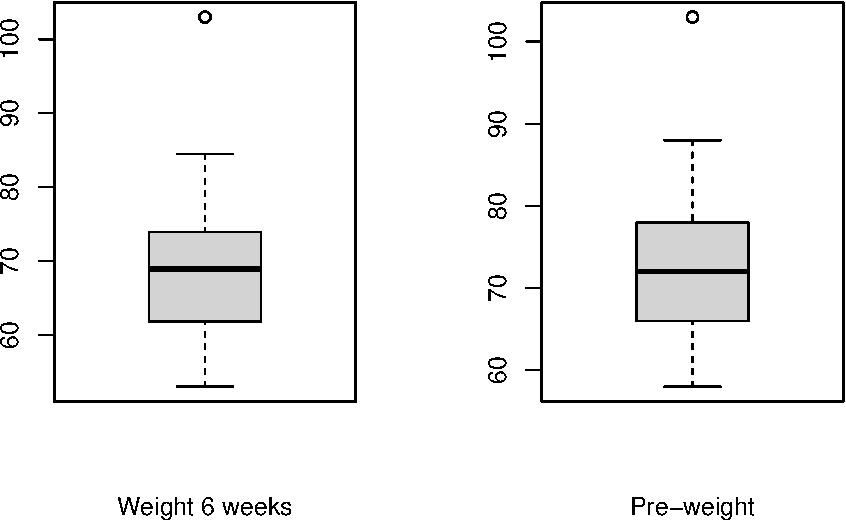
\includegraphics{assignment_1_files/figure-latex/unnamed-chunk-21-1.pdf}

\begin{Shaded}
\begin{Highlighting}[]
\CommentTok{\#Check for if data is normaly distributed}
\FunctionTok{hist}\NormalTok{(diet}\SpecialCharTok{$}\NormalTok{weight6weeks }\SpecialCharTok{{-}}\NormalTok{ diet}\SpecialCharTok{$}\NormalTok{preweight, }\AttributeTok{main =} \StringTok{"Difference in weight after 6 weeks"}\NormalTok{, }\AttributeTok{xlab =} \StringTok{"Difference"}\NormalTok{)}
\FunctionTok{qqnorm}\NormalTok{(diet}\SpecialCharTok{$}\NormalTok{weight6weeks }\SpecialCharTok{{-}}\NormalTok{ diet}\SpecialCharTok{$}\NormalTok{preweight)}
\FunctionTok{qqline}\NormalTok{(diet}\SpecialCharTok{$}\NormalTok{weight6weeks }\SpecialCharTok{{-}}\NormalTok{ diet}\SpecialCharTok{$}\NormalTok{preweight)}
\end{Highlighting}
\end{Shaded}

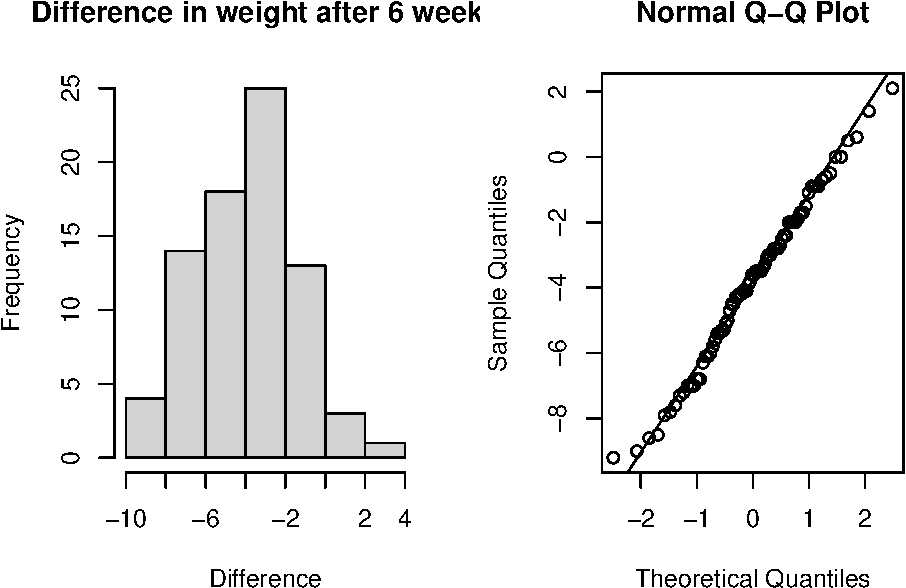
\includegraphics{assignment_1_files/figure-latex/unnamed-chunk-21-2.pdf}

\begin{Shaded}
\begin{Highlighting}[]
\FunctionTok{t.test}\NormalTok{(diet}\SpecialCharTok{$}\NormalTok{preweight, diet}\SpecialCharTok{$}\NormalTok{weight6weeks, }\AttributeTok{paired =} \ConstantTok{TRUE}\NormalTok{)}
\end{Highlighting}
\end{Shaded}

\begin{verbatim}
## 
##  Paired t-test
## 
## data:  diet$preweight and diet$weight6weeks
## t = 13.309, df = 77, p-value < 2.2e-16
## alternative hypothesis: true mean difference is not equal to 0
## 95 percent confidence interval:
##  3.269602 4.420141
## sample estimates:
## mean difference 
##        3.844872
\end{verbatim}

\textbf{b)}

Our goal is to use one-way ANOVA test to compare the diets. We first
draw QQ-plot to check if we can assume normality this seems to be the
case so we perform ANOVA with the Hypotheses:

\begin{itemize}
\item
  Null hypothesis (H0): The means of the lost weight are equal among the
  three types of diets.
\item
  Alternative hypothesis (Ha): The mean of at least one diet-type is not
  equal among the three types of diets.
\end{itemize}

The ANOVA

Looking at the summary of the anova table we can see clearly that the
p-value of diet 3 is smaller than our significance level of 0.05.
Therefor we reject the null hypothesis and assume that there is a
difference between the diets. All diets have and effect this is shown in
question a. Diet 3 has the biggest effect on the weight lost.

The Kruskal-Wallis is also valid because it has the same pre-conditions
as the anova test the difference is that Kruskal-Wallis test can also be
used when normality cannot be assumed.

\begin{Shaded}
\begin{Highlighting}[]
\NormalTok{dietframe }\OtherTok{\textless{}{-}} \FunctionTok{data.frame}\NormalTok{(}\AttributeTok{weight=}\NormalTok{(diet}\SpecialCharTok{$}\NormalTok{preweight}\SpecialCharTok{{-}}\NormalTok{diet}\SpecialCharTok{$}\NormalTok{weight6weeks), }\AttributeTok{diet=}\FunctionTok{factor}\NormalTok{(diet}\SpecialCharTok{$}\NormalTok{diet))}
\NormalTok{dietanov}\OtherTok{=}\FunctionTok{lm}\NormalTok{(weight}\SpecialCharTok{\textasciitilde{}}\NormalTok{diet ,}\AttributeTok{data =}\NormalTok{ dietframe)}
\FunctionTok{anova}\NormalTok{(dietanov)}
\end{Highlighting}
\end{Shaded}

\begin{verbatim}
## Analysis of Variance Table
## 
## Response: weight
##           Df Sum Sq Mean Sq F value   Pr(>F)   
## diet       2  71.09  35.547  6.1974 0.003229 **
## Residuals 75 430.18   5.736                    
## ---
## Signif. codes:  0 '***' 0.001 '**' 0.01 '*' 0.05 '.' 0.1 ' ' 1
\end{verbatim}

\begin{Shaded}
\begin{Highlighting}[]
\FunctionTok{summary}\NormalTok{(dietanov)}
\end{Highlighting}
\end{Shaded}

\begin{verbatim}
## 
## Call:
## lm(formula = weight ~ diet, data = dietframe)
## 
## Residuals:
##     Min      1Q  Median      3Q     Max 
## -5.1259 -1.3815  0.1759  1.6519  5.7000 
## 
## Coefficients:
##             Estimate Std. Error t value Pr(>|t|)    
## (Intercept)   3.3000     0.4889   6.750 2.72e-09 ***
## diet2        -0.2741     0.6719  -0.408  0.68449    
## diet3         1.8481     0.6719   2.751  0.00745 ** 
## ---
## Signif. codes:  0 '***' 0.001 '**' 0.01 '*' 0.05 '.' 0.1 ' ' 1
## 
## Residual standard error: 2.395 on 75 degrees of freedom
## Multiple R-squared:  0.1418, Adjusted R-squared:  0.1189 
## F-statistic: 6.197 on 2 and 75 DF,  p-value: 0.003229
\end{verbatim}

\begin{Shaded}
\begin{Highlighting}[]
\FunctionTok{par}\NormalTok{(}\AttributeTok{mfrow=}\FunctionTok{c}\NormalTok{(}\DecValTok{1}\NormalTok{,}\DecValTok{2}\NormalTok{)); }\FunctionTok{qqnorm}\NormalTok{(}\FunctionTok{residuals}\NormalTok{(dietanov))}
\FunctionTok{qqline}\NormalTok{(}\FunctionTok{residuals}\NormalTok{(dietanov))}
\FunctionTok{plot}\NormalTok{(}\FunctionTok{fitted}\NormalTok{(dietanov),}\FunctionTok{residuals}\NormalTok{(dietanov))}
\end{Highlighting}
\end{Shaded}

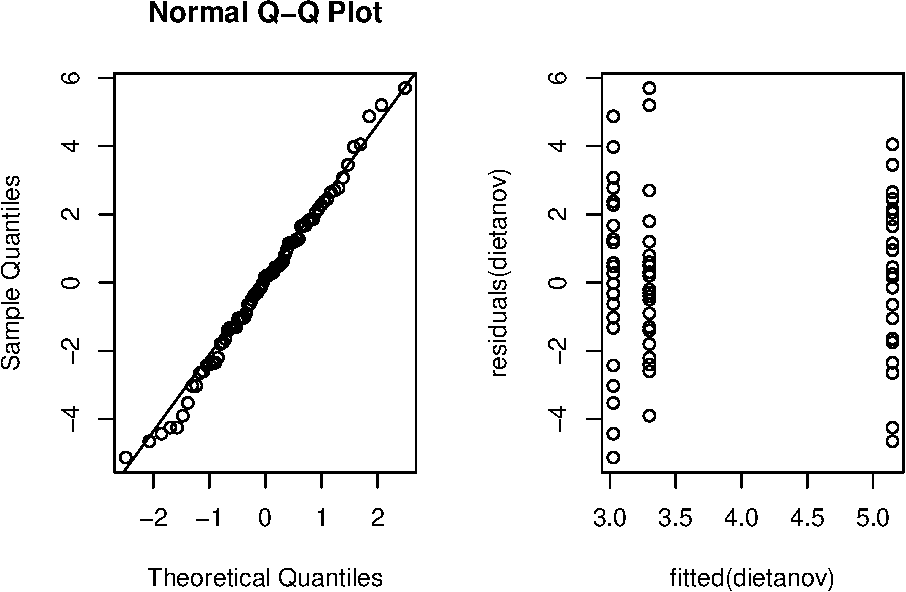
\includegraphics{assignment_1_files/figure-latex/unnamed-chunk-22-1.pdf}

\textbf{c )}

Our goal is to use two-way ANOVA test to investigate the effects on
gender and different diets on the mean lost weight. We first draw
QQ-plot to check if we can assume normality this seems to be the case so
we can go over to our hypothesis.

\begin{itemize}
\item
  Null hypothesis (H0): The means of the lost weight are equal among the
  factors.
\item
  Alternative hypothesis (Ha): The means of the lost weight are not
  equal for at least one factor.
\end{itemize}

The result of the ANOVA test is that we can reject the null hypothesis.
There is a difference between the means of the lost weight. There also
is a small significant interaction between diet and gender with a
p-value of \textasciitilde0.048. Looking at the summary we can see that
this is not a specific interaction between a specific diet type and
gender but a general effect that gender has on all diet types.

\begin{Shaded}
\begin{Highlighting}[]
\NormalTok{dgframe }\OtherTok{\textless{}{-}} \FunctionTok{data.frame}\NormalTok{(}\AttributeTok{weight=}\NormalTok{diet}\SpecialCharTok{$}\NormalTok{preweight }\SpecialCharTok{{-}}\NormalTok{ diet}\SpecialCharTok{$}\NormalTok{weight6weeks, }\AttributeTok{diet=}\FunctionTok{factor}\NormalTok{(diet}\SpecialCharTok{$}\NormalTok{diet), }\AttributeTok{gender=}\FunctionTok{factor}\NormalTok{(diet}\SpecialCharTok{$}\NormalTok{gender))}
\NormalTok{dganov}\OtherTok{=}\FunctionTok{lm}\NormalTok{(weight}\SpecialCharTok{\textasciitilde{}}\NormalTok{diet}\SpecialCharTok{*}\NormalTok{gender ,}\AttributeTok{data =}\NormalTok{ dgframe)}
\FunctionTok{anova}\NormalTok{(dganov)}
\end{Highlighting}
\end{Shaded}

\begin{verbatim}
## Analysis of Variance Table
## 
## Response: weight
##             Df Sum Sq Mean Sq F value   Pr(>F)   
## diet         2  60.53 30.2635  5.6292 0.005408 **
## gender       1   0.17  0.1687  0.0314 0.859910   
## diet:gender  2  33.90 16.9520  3.1532 0.048842 * 
## Residuals   70 376.33  5.3761                    
## ---
## Signif. codes:  0 '***' 0.001 '**' 0.01 '*' 0.05 '.' 0.1 ' ' 1
\end{verbatim}

\begin{Shaded}
\begin{Highlighting}[]
\FunctionTok{summary}\NormalTok{(dganov)}
\end{Highlighting}
\end{Shaded}

\begin{verbatim}
## 
## Call:
## lm(formula = weight ~ diet * gender, data = dgframe)
## 
## Residuals:
##     Min      1Q  Median      3Q     Max 
## -5.5091 -1.2958  0.0705  1.2159  5.4500 
## 
## Coefficients:
##               Estimate Std. Error t value Pr(>|t|)    
## (Intercept)     3.0500     0.6197   4.922 5.49e-06 ***
## diet2          -0.4429     0.8764  -0.505   0.6149    
## diet3           2.8300     0.8616   3.284   0.0016 ** 
## gender1         0.6000     0.9600   0.625   0.5340    
## diet2:gender1   0.9019     1.3395   0.673   0.5030    
## diet3:gender1  -2.2467     1.3145  -1.709   0.0919 .  
## ---
## Signif. codes:  0 '***' 0.001 '**' 0.01 '*' 0.05 '.' 0.1 ' ' 1
## 
## Residual standard error: 2.319 on 70 degrees of freedom
##   (2 observations deleted due to missingness)
## Multiple R-squared:  0.2009, Adjusted R-squared:  0.1438 
## F-statistic: 3.519 on 5 and 70 DF,  p-value: 0.006775
\end{verbatim}

\begin{Shaded}
\begin{Highlighting}[]
\FunctionTok{par}\NormalTok{(}\AttributeTok{mfrow=}\FunctionTok{c}\NormalTok{(}\DecValTok{1}\NormalTok{,}\DecValTok{2}\NormalTok{))}
\FunctionTok{qqnorm}\NormalTok{(}\FunctionTok{residuals}\NormalTok{(dganov))}
\FunctionTok{plot}\NormalTok{(}\FunctionTok{fitted}\NormalTok{(dganov), }\FunctionTok{residuals}\NormalTok{(dganov))}
\end{Highlighting}
\end{Shaded}

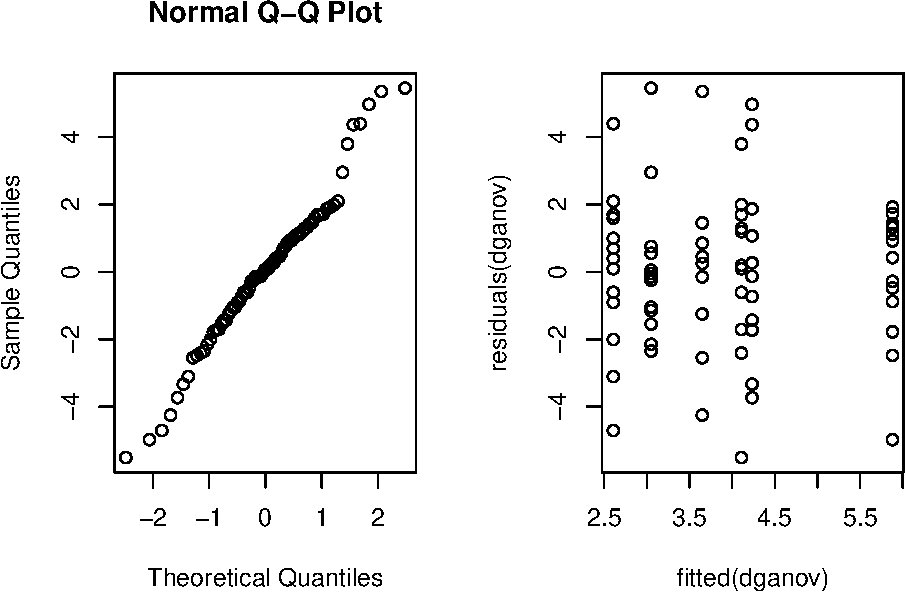
\includegraphics{assignment_1_files/figure-latex/unnamed-chunk-23-1.pdf}

\textbf{e )}

Whether we want to use one-way or two-way ANOVA depends on what we want
to investigate. If we want to see the effects of different diets on
weight loss one-way ANOVA would be sufficient. However if we are
interested in the effect of gender on the effectiveness of diet this
one-way model could not work. Therefor we would have to use two-way
ANOVA. Because we only want to predict the lost weight achieved by
diet-type we are going to use the same linear model we used for one-way
ANOVA to predict weight loss for the different diet-types.

\begin{Shaded}
\begin{Highlighting}[]
\FunctionTok{summary}\NormalTok{(dietanov)}
\end{Highlighting}
\end{Shaded}

\begin{verbatim}
## 
## Call:
## lm(formula = weight ~ diet, data = dietframe)
## 
## Residuals:
##     Min      1Q  Median      3Q     Max 
## -5.1259 -1.3815  0.1759  1.6519  5.7000 
## 
## Coefficients:
##             Estimate Std. Error t value Pr(>|t|)    
## (Intercept)   3.3000     0.4889   6.750 2.72e-09 ***
## diet2        -0.2741     0.6719  -0.408  0.68449    
## diet3         1.8481     0.6719   2.751  0.00745 ** 
## ---
## Signif. codes:  0 '***' 0.001 '**' 0.01 '*' 0.05 '.' 0.1 ' ' 1
## 
## Residual standard error: 2.395 on 75 degrees of freedom
## Multiple R-squared:  0.1418, Adjusted R-squared:  0.1189 
## F-statistic: 6.197 on 2 and 75 DF,  p-value: 0.003229
\end{verbatim}

Looking at the summary for the ANOVA model we can see that the estimate
average weight difference between the before and after. This would mean
that the prediction for the weight loss after 6 weeks will be:

\begin{longtable}[]{@{}ll@{}}
\toprule()
Col1 & Col2 \\
\midrule()
\endhead
diet 1 & 3.3 kg \\
diet 2 & 3.1 kg \\
diet 3 & 5.1 kg \\
\bottomrule()
\end{longtable}

\hypertarget{exercise-4}{%
\subsection{Exercise 4}\label{exercise-4}}

\begin{Shaded}
\begin{Highlighting}[]
\NormalTok{npk}
\end{Highlighting}
\end{Shaded}

\begin{verbatim}
##    block N P K yield
## 1      1 0 1 1  49.5
## 2      1 1 1 0  62.8
## 3      1 0 0 0  46.8
## 4      1 1 0 1  57.0
## 5      2 1 0 0  59.8
## 6      2 1 1 1  58.5
## 7      2 0 0 1  55.5
## 8      2 0 1 0  56.0
## 9      3 0 1 0  62.8
## 10     3 1 1 1  55.8
## 11     3 1 0 0  69.5
## 12     3 0 0 1  55.0
## 13     4 1 0 0  62.0
## 14     4 1 1 1  48.8
## 15     4 0 0 1  45.5
## 16     4 0 1 0  44.2
## 17     5 1 1 0  52.0
## 18     5 0 0 0  51.5
## 19     5 1 0 1  49.8
## 20     5 0 1 1  48.8
## 21     6 1 0 1  57.2
## 22     6 1 1 0  59.0
## 23     6 0 1 1  53.2
## 24     6 0 0 0  56.0
\end{verbatim}

\textbf{a)}

We loop over all the blocks and sample 2 plots for each additive.

\begin{Shaded}
\begin{Highlighting}[]
\CommentTok{\#randomized plot design}
\NormalTok{plot}\OtherTok{=}\FunctionTok{c}\NormalTok{(}\DecValTok{0}\NormalTok{,}\DecValTok{1}\NormalTok{,}\DecValTok{2}\NormalTok{,}\DecValTok{3}\NormalTok{)}
\NormalTok{plots }\OtherTok{=} \FunctionTok{data.frame}\NormalTok{(}\FunctionTok{matrix}\NormalTok{(}\DecValTok{0}\NormalTok{, }\AttributeTok{ncol =} \DecValTok{4}\NormalTok{, }\AttributeTok{nrow =} \DecValTok{24}\NormalTok{))}
\ControlFlowTok{for}\NormalTok{(i }\ControlFlowTok{in} \DecValTok{1}\SpecialCharTok{:}\DecValTok{24}\NormalTok{)\{}
  \ControlFlowTok{if}\NormalTok{(i }\SpecialCharTok{\%\%} \DecValTok{4} \SpecialCharTok{!=} \DecValTok{1}\NormalTok{)\{}\ControlFlowTok{next}\NormalTok{\}}
  
\NormalTok{  x}\OtherTok{\textless{}{-}}\FunctionTok{as.integer}\NormalTok{(i}\SpecialCharTok{/}\DecValTok{4}\NormalTok{)}\SpecialCharTok{+}\DecValTok{1}
\NormalTok{  plots[i, }\DecValTok{4}\NormalTok{]}\OtherTok{=}\NormalTok{ x}
\NormalTok{  plots[i}\SpecialCharTok{+}\DecValTok{1}\NormalTok{, }\DecValTok{4}\NormalTok{]}\OtherTok{=}\NormalTok{ x}
\NormalTok{  plots[i}\SpecialCharTok{+}\DecValTok{2}\NormalTok{, }\DecValTok{4}\NormalTok{]}\OtherTok{=}\NormalTok{ x}
\NormalTok{  plots[i}\SpecialCharTok{+}\DecValTok{3}\NormalTok{, }\DecValTok{4}\NormalTok{]}\OtherTok{=}\NormalTok{ x}
  
  \ControlFlowTok{for}\NormalTok{(j }\ControlFlowTok{in} \DecValTok{1}\SpecialCharTok{:}\DecValTok{3}\NormalTok{)\{}
\NormalTok{    sample\_plots }\OtherTok{=} \FunctionTok{sample}\NormalTok{(plot, }\DecValTok{2}\NormalTok{)}
\NormalTok{    plots[i}\SpecialCharTok{+}\NormalTok{sample\_plots[}\DecValTok{1}\NormalTok{],j] }\OtherTok{=} \DecValTok{1}
\NormalTok{    plots[i}\SpecialCharTok{+}\NormalTok{sample\_plots[}\DecValTok{2}\NormalTok{],j] }\OtherTok{=} \DecValTok{1}
\NormalTok{  \}}
\NormalTok{\}}
\FunctionTok{colnames}\NormalTok{(plots) }\OtherTok{=} \FunctionTok{c}\NormalTok{(}\StringTok{"N"}\NormalTok{,}\StringTok{"P"}\NormalTok{, }\StringTok{"K"}\NormalTok{, }\StringTok{"Blocks"}\NormalTok{)}
\NormalTok{plots}
\end{Highlighting}
\end{Shaded}

\begin{verbatim}
##    N P K Blocks
## 1  0 0 1      1
## 2  1 1 0      1
## 3  1 0 1      1
## 4  0 1 0      1
## 5  0 0 1      2
## 6  1 1 1      2
## 7  0 0 0      2
## 8  1 1 0      2
## 9  0 1 0      3
## 10 0 1 0      3
## 11 1 0 1      3
## 12 1 0 1      3
## 13 0 1 0      4
## 14 1 0 0      4
## 15 0 0 1      4
## 16 1 1 1      4
## 17 1 0 0      5
## 18 1 0 1      5
## 19 0 1 0      5
## 20 0 1 1      5
## 21 1 0 0      6
## 22 0 0 1      6
## 23 1 1 0      6
## 24 0 1 1      6
\end{verbatim}

\textbf{b)}

By looking at every block you get a more precise picture of the
different combinations. Because different blocks have different
combinations of additives applied. This way you can determine the effect
the other additives have on the yield.

\begin{Shaded}
\begin{Highlighting}[]
\FunctionTok{par}\NormalTok{(}\AttributeTok{mfrow=}\FunctionTok{c}\NormalTok{(}\DecValTok{1}\NormalTok{,}\DecValTok{2}\NormalTok{))}
\FunctionTok{interaction.plot}\NormalTok{(npk}\SpecialCharTok{$}\NormalTok{N, npk}\SpecialCharTok{$}\NormalTok{block, npk}\SpecialCharTok{$}\NormalTok{yield, }\AttributeTok{xlab =} \StringTok{"nitrogen"}\NormalTok{, }\AttributeTok{ylab =} \StringTok{"yield"}\NormalTok{, }\AttributeTok{trace.label =} \StringTok{"block"}\NormalTok{)}
\FunctionTok{interaction.plot}\NormalTok{(npk}\SpecialCharTok{$}\NormalTok{block, npk}\SpecialCharTok{$}\NormalTok{N, npk}\SpecialCharTok{$}\NormalTok{yield, }\AttributeTok{xlab =} \StringTok{"block"}\NormalTok{, }\AttributeTok{ylab =} \StringTok{"yield"}\NormalTok{, }\AttributeTok{trace.label =} \StringTok{"nitrogen"}\NormalTok{)}
\end{Highlighting}
\end{Shaded}

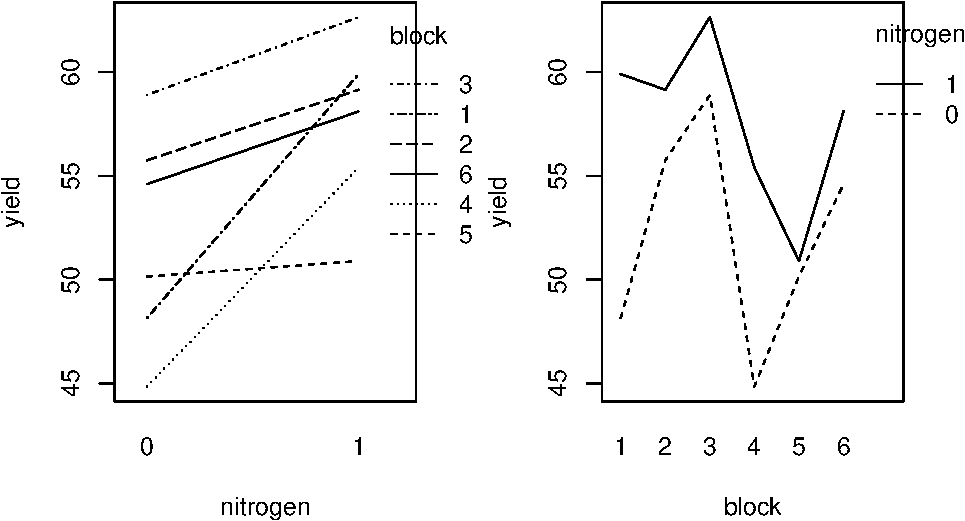
\includegraphics{assignment_1_files/figure-latex/unnamed-chunk-27-1.pdf}

\textbf{c)}

\begin{itemize}
\item
  Null hypothesis: The means of the yield are equal among the factors.
\item
  Alternative hypothesis: The means of the yield are not equal for at
  least one factor.
\end{itemize}

The p-value for block is not significant therefore we cannot reject H0.
The p-value for nitrogen is significant however and that means we can
reject H0 and accept Ha. It is sensible to include the block factor in
the model because the yield is source of variation by including it we
can account for this variation and better estimate the effect nitrogen.

The Friedman test can't be used because the Friedman test is
non-parametric test for comparing two groups on a dependent variable.
However here we have two groups and a response variable.

\begin{Shaded}
\begin{Highlighting}[]
\NormalTok{npk}\SpecialCharTok{$}\NormalTok{block }\OtherTok{=} \FunctionTok{as.factor}\NormalTok{(npk}\SpecialCharTok{$}\NormalTok{block)}
\NormalTok{npk}\SpecialCharTok{$}\NormalTok{N }\OtherTok{=} \FunctionTok{as.factor}\NormalTok{(npk}\SpecialCharTok{$}\NormalTok{N)}

\NormalTok{npkanov }\OtherTok{=} \FunctionTok{lm}\NormalTok{(yield}\SpecialCharTok{\textasciitilde{}}\NormalTok{block}\SpecialCharTok{*}\NormalTok{N, }\AttributeTok{data=}\NormalTok{npk)}
\FunctionTok{anova}\NormalTok{(npkanov)}
\end{Highlighting}
\end{Shaded}

\begin{verbatim}
## Analysis of Variance Table
## 
## Response: yield
##           Df Sum Sq Mean Sq F value  Pr(>F)  
## block      5 343.30  68.659  3.3592 0.03967 *
## N          1 189.28 189.282  9.2607 0.01021 *
## block:N    5  98.52  19.704  0.9640 0.47690  
## Residuals 12 245.27  20.439                  
## ---
## Signif. codes:  0 '***' 0.001 '**' 0.01 '*' 0.05 '.' 0.1 ' ' 1
\end{verbatim}

\begin{Shaded}
\begin{Highlighting}[]
\FunctionTok{summary}\NormalTok{(npkanov)}
\end{Highlighting}
\end{Shaded}

\begin{verbatim}
## 
## Call:
## lm(formula = yield ~ block * N, data = npk)
## 
## Residuals:
##    Min     1Q Median     3Q    Max 
##  -6.85  -1.35   0.00   1.35   6.85 
## 
## Coefficients:
##             Estimate Std. Error t value Pr(>|t|)    
## (Intercept)   48.150      3.197  15.062 3.71e-09 ***
## block2         7.600      4.521   1.681   0.1186    
## block3        10.750      4.521   2.378   0.0349 *  
## block4        -3.300      4.521  -0.730   0.4794    
## block5         2.000      4.521   0.442   0.6661    
## block6         6.450      4.521   1.427   0.1792    
## N1            11.750      4.521   2.599   0.0233 *  
## block2:N1     -8.350      6.394  -1.306   0.2160    
## block3:N1     -8.000      6.394  -1.251   0.2347    
## block4:N1     -1.200      6.394  -0.188   0.8543    
## block5:N1    -11.000      6.394  -1.720   0.1110    
## block6:N1     -8.250      6.394  -1.290   0.2212    
## ---
## Signif. codes:  0 '***' 0.001 '**' 0.01 '*' 0.05 '.' 0.1 ' ' 1
## 
## Residual standard error: 4.521 on 12 degrees of freedom
## Multiple R-squared:  0.7201, Adjusted R-squared:  0.4636 
## F-statistic: 2.807 on 11 and 12 DF,  p-value: 0.04492
\end{verbatim}

\begin{Shaded}
\begin{Highlighting}[]
\FunctionTok{par}\NormalTok{(}\AttributeTok{mfrow=}\FunctionTok{c}\NormalTok{(}\DecValTok{1}\NormalTok{,}\DecValTok{2}\NormalTok{))}
\FunctionTok{qqnorm}\NormalTok{(}\FunctionTok{residuals}\NormalTok{(npkanov))}
\FunctionTok{plot}\NormalTok{(}\FunctionTok{fitted}\NormalTok{(npkanov), }\FunctionTok{residuals}\NormalTok{(npkanov))}
\end{Highlighting}
\end{Shaded}

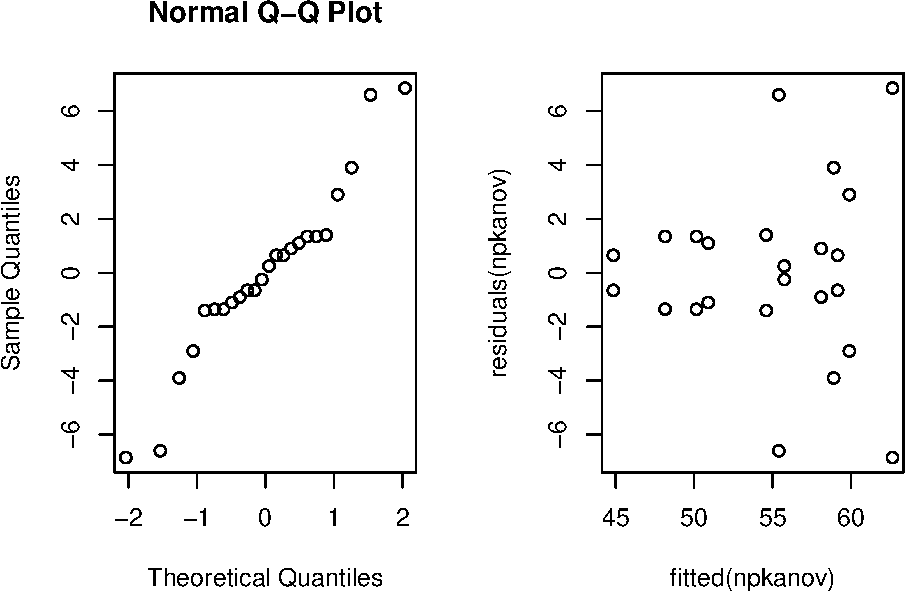
\includegraphics{assignment_1_files/figure-latex/unnamed-chunk-28-1.pdf}

\textbf{d)}

We did a investigation on the significance of the variables. And removed
each iteration the least significant value from the model. At the end we
only had Nitrogen left and because it the only factor with significance
relation we have chosen it as our favorite.

\begin{Shaded}
\begin{Highlighting}[]
\NormalTok{npk}\SpecialCharTok{$}\NormalTok{block }\OtherTok{=} \FunctionTok{as.factor}\NormalTok{(npk}\SpecialCharTok{$}\NormalTok{block)}
\NormalTok{npk}\SpecialCharTok{$}\NormalTok{N }\OtherTok{=} \FunctionTok{as.factor}\NormalTok{(npk}\SpecialCharTok{$}\NormalTok{N)}
\NormalTok{npk}\SpecialCharTok{$}\NormalTok{P }\OtherTok{=} \FunctionTok{as.factor}\NormalTok{(npk}\SpecialCharTok{$}\NormalTok{P)}
\NormalTok{npk}\SpecialCharTok{$}\NormalTok{K }\OtherTok{=} \FunctionTok{as.factor}\NormalTok{(npk}\SpecialCharTok{$}\NormalTok{K)}

\NormalTok{giganov }\OtherTok{=} \FunctionTok{lm}\NormalTok{(yield}\SpecialCharTok{\textasciitilde{}}\NormalTok{block}\SpecialCharTok{+}\NormalTok{N}\SpecialCharTok{+}\NormalTok{P}\SpecialCharTok{+}\NormalTok{K, }\AttributeTok{data =}\NormalTok{ npk)}
\FunctionTok{anova}\NormalTok{(giganov)}
\end{Highlighting}
\end{Shaded}

\begin{verbatim}
## Analysis of Variance Table
## 
## Response: yield
##           Df Sum Sq Mean Sq F value  Pr(>F)   
## block      5 343.30  68.659  4.2879 0.01272 * 
## N          1 189.28 189.282 11.8210 0.00366 **
## P          1   8.40   8.402  0.5247 0.47999   
## K          1  95.20  95.202  5.9455 0.02767 * 
## Residuals 15 240.19  16.012                   
## ---
## Signif. codes:  0 '***' 0.001 '**' 0.01 '*' 0.05 '.' 0.1 ' ' 1
\end{verbatim}

\begin{Shaded}
\begin{Highlighting}[]
\FunctionTok{par}\NormalTok{(}\AttributeTok{mfrow=}\FunctionTok{c}\NormalTok{(}\DecValTok{1}\NormalTok{,}\DecValTok{2}\NormalTok{))}
\FunctionTok{qqnorm}\NormalTok{(}\FunctionTok{residuals}\NormalTok{(giganov))}
\FunctionTok{plot}\NormalTok{(}\FunctionTok{fitted}\NormalTok{(giganov), }\FunctionTok{residuals}\NormalTok{(giganov))}
\end{Highlighting}
\end{Shaded}

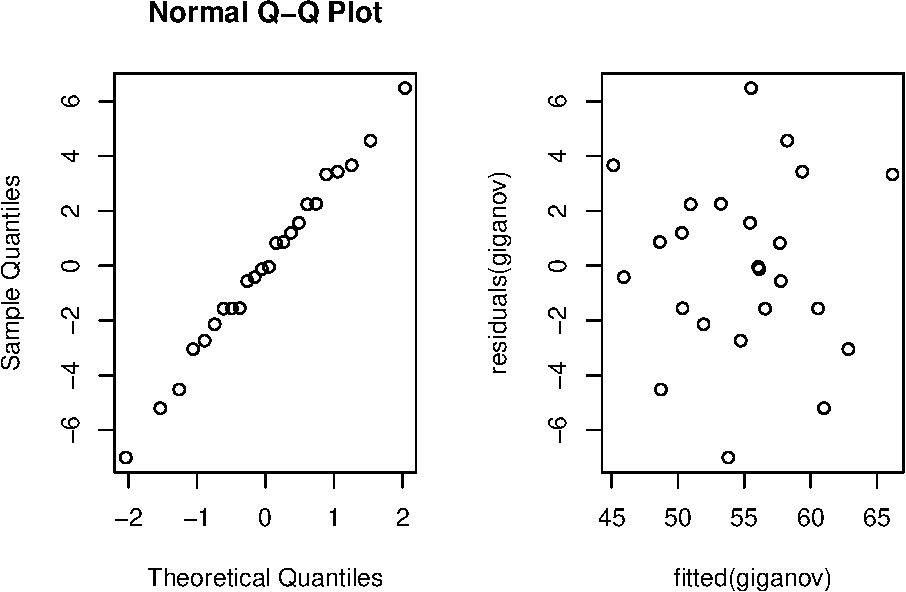
\includegraphics{assignment_1_files/figure-latex/unnamed-chunk-29-1.pdf}

\begin{Shaded}
\begin{Highlighting}[]
\NormalTok{model1 }\OtherTok{=} \FunctionTok{lm}\NormalTok{(yield}\SpecialCharTok{\textasciitilde{}}\NormalTok{block}\SpecialCharTok{+}\NormalTok{N}\SpecialCharTok{+}\NormalTok{K, }\AttributeTok{data =}\NormalTok{ npk)}
\FunctionTok{anova}\NormalTok{(model1)}
\end{Highlighting}
\end{Shaded}

\begin{verbatim}
## Analysis of Variance Table
## 
## Response: yield
##           Df Sum Sq Mean Sq F value   Pr(>F)   
## block      5 343.30  68.659  4.4192 0.010172 * 
## N          1 189.28 189.282 12.1829 0.003024 **
## K          1  95.20  95.202  6.1275 0.024874 * 
## Residuals 16 248.59  15.537                    
## ---
## Signif. codes:  0 '***' 0.001 '**' 0.01 '*' 0.05 '.' 0.1 ' ' 1
\end{verbatim}

\begin{Shaded}
\begin{Highlighting}[]
\NormalTok{model2 }\OtherTok{=} \FunctionTok{lm}\NormalTok{(yield}\SpecialCharTok{\textasciitilde{}}\NormalTok{block}\SpecialCharTok{+}\NormalTok{N, }\AttributeTok{data =}\NormalTok{ npk)}
\FunctionTok{anova}\NormalTok{(model2)}
\end{Highlighting}
\end{Shaded}

\begin{verbatim}
## Analysis of Variance Table
## 
## Response: yield
##           Df Sum Sq Mean Sq F value   Pr(>F)   
## block      5 343.30  68.659  3.3951 0.026173 * 
## N          1 189.28 189.282  9.3598 0.007095 **
## Residuals 17 343.79  20.223                    
## ---
## Signif. codes:  0 '***' 0.001 '**' 0.01 '*' 0.05 '.' 0.1 ' ' 1
\end{verbatim}

\textbf{e)}

The output of the mixed effect analysis will generally return a smaller
standard error than that of the fixed effects model because the mixed
effects model also accounts for variation that is caused by the
difference of the blocks. Furthermore we can use the random effect of
the block to estimate the variance in yield.

\begin{Shaded}
\begin{Highlighting}[]
\CommentTok{\# library(lme4.0)}
\CommentTok{\# npklmer=lmer(yield \textasciitilde{} N + (1|block), data = npk)}
\CommentTok{\# summary}
\end{Highlighting}
\end{Shaded}


\end{document}
